\newpage
\subsection{Учет технологической оснастки }
\label{bp:rigging}
%
Технологическая оснастка необходима для изготовления готовой продукции. На предприятии заказывают оснастку у сторонних производителей. Изготовление штанцевальных форм осуществляет ООО «РАСТР—технология». Ротационные штанцевальные формы заказываются в г. Москва. Плоские штанцевальные формы заказываются в г. Новосибирск. Изготовление флекс-форм осуществляет ООО "Аверс" г. Барнаул. 

При получении требований от клиента менеджер узнает о необходимости использования оснастки при производстве продукции. 

Возможность изготовления нового изделия на производстве определяет менеджер по согласованию с главным технологом.
%Если МСЗ сомневается в возможности производства продукции, он задает вопрос на производство инженеру-технологу или директору по  производству. 

\textbf{Учет печатных форм}

Дизайнера в штате предприятия нет.
Менеджер заказывает разработку дизайна и изготовление печатной флекс-формы в ООО "Аверс" г. Барнаул. 
На выходе компания ООО "Аверс" разрабатывает макет (форма \ref{pic:d17}). Менеджер исправляет в программе Paint в форме \ref{pic:d17} данные по ТК.
Менеджер запрашивает макет для печати на изделии (форма \ref{pic:d16}).

Разработка дизайна для печатных форм на предприятии не осуществляется.  
Предприятие использует одного поставщика флекс-форм. 
Для заказа флекс-формы менеджер использует  дизайн макет и отправляет его по электронной почте производителю оснастки после проверки главным технологом.%, заявку на изготовление флекс-формы. 
%МСЗ и МАП проверяют внешний вид печати в файле согласованной технологической карты.

 Менеджер готовит служебную записку на приобретение оснастки. Служебную записку согласовывает генеральный директор. Менеджер отправляет документ по электронной почте производителю оснастки.
%При изготовлении печатной флекс-формы за счет клиента менеджер выставляет счет на изготовление оснастки.

При поступлении на производство оснастка проверяется главным технологом совместно с контролером по качеству. В ближайшее время функционал по работе с оснасткой планируется передать инженеру по подготовке производства. На основании приходных документов бухгалтер ставит оснастку на учет в системе 1С:Бухгалтерия предприятия.  

%Номер печатной формы присваивает участок вырубных форм на производстве в момент первого запуска и при нахождении свободной ячейки для хранения (рис. \ref{pic:f44}).  
Номер флекс-формы присваивается производителем и в дальнейшем используется на предприятии. Номер и наименование записываются в файле  MS Excel, где ведется список используемых на предприятии флекс-форм. Печатный вариант списка с указанием наименований находится в месте хранения оснастки (рис. \ref{pic:1/6 перечень оснастки}). 
Мелкий ремонт флекс-форм производят машинисты на линиях переработки.

На предприятии выделено место хранения флекс-форм (рис. \ref{pic:1/6 хранение фпф}).
При появлении заданий от специалиста по планированию в  MS Excel контролеры по качеству ежесменно проверяют физическое наличие и целостность клише и готовят к выдаче  на специальном столе. Операторы линий переработки забирают нужные флекс-формы, а затем в конце смены возвращают их для промывки и дальнейшего хранения. Контролеры по качеству промывают флекс-формы и возвращают их на соответствующие места хранения.
Журнала выдачи оснастки не обнаружено.
%, 32, 33При появлении заданий от специалиста по планированию в Excel контролеры по качеству проверяют физическое наличие и целостность клише и готовят к выдаче  на специальном столе. Операторы линий переработки забирают нужные флекс-формы, а затем в конце смены возвращают их для промывки и дальнейшего хранения. Контролеры по качеству промывают флекс-формы и возвращают их на соответствующие места хранения.
%Журнала выдачи оснастки не обнаружено.
%При поступлении оснастки МСЗ принимает ее совместно с комплектовщиком, проверяют качество, присваивают номер.
%Номер определяется по файлу в формате MS Excel, где ведется список используемых на предприятии флекс-форм.

%После принятия к учету флекс-форм МСЗ сообщает дизайнеру о поступлении устно или через мессенджеры о необходимости добавления номера поступившей оснастки в разработанную технологическую карту.
%Комплектовщик принимает флекс-форму и размещает в ячейке для хранения. Место хранения флексо-форм  разделено по линиям (\ref{pic:a15}).  


\textbf{Учет штанцевальных форм.}

На предприятии используются роторные и плоские высекательные штанцевальные формы.

%Клиент предоставляет макет по изготовлению изделия для сложных изделий. Дизайнер на предприятии не разрабатывает макет высекательных штанцевальных форм.


Штанцевальные формы разрабатывает ООО «РАСТР—технология».
Макет разрабатывается главным технологом по запросу менеджера. 
Главный технолог высылает согласованный чертеж по почте в компанию-изготовитель.
Изготовитель штанцевальной формы корректирует чертеж по своим правилам, высылает обратно на согласование. Менеджер готовит служебную записку на приобретение оснастки (рис. \ref{pic:1.8 приобретение оснастки_0001}). Служебную записку согласовывает генеральный директор. Менеджер отправляет документ по электронной почте производителю оснастки.% Если изготовление штанцевальной формы выполняется за счет клиента, то менеджер выставляет счет покупателю.

При поступлении штампа на производство главный технолог  проверяет его визуально и определяет место хранения. Для идентификации штанцевальной формы используется номер присвоенный производителем. Номер и наименование записываются в файле  MS Excel, где ведется список используемых на предприятии штанцевальных форм. На основании приходных документов бухгалтер ставит оснастку на учет в системе 1С: ''Бухгалтерия предприятия''. Ремонт штампов на предприятии не производится (исключение мелкий ремонт). 
На предприятии у каждой линии переработки выделено место для хранения штампов.  (рис. \ref{pic:1/6 хранение штанцев}).
Машинист при настройке на задание сам находит и берет штамп с места хранения и устанавливает на линию. Журнала учета выдачи оснастки не выявлено. После выработки задания машинист  возвращает штампы на место. При необходимости производится мелкий ремонт силами бригады. Записи по проведению ремонтов не ведутся. 
%Номер и место присваивается после первого пуска. Места хранения штанцев на стеллажах распределены по контрагентам. 
Учет пробега по оснастке осуществляет главный технолог в файле MS EXCEL и отчитывается перед генеральным директором. Учет ведется не по всем позициям. Расчет пробега ведется на основании информации из бухгалтерии.
%Ремонтом штампов занимается участок вырубных форм при обнаружении неисправности. Ремонтируют только резинки и прямые ножи. 
\clearpage

%При поступлении штанцевальной формы МСЗ принимает ее вместе с комплектовщиком, проверяет качество. 
%Комплектовщик присваивает номер штанцевальной формы согласно файла реестра штанцевальной формы (рис. \ref{pic:d10}), сообщает дизайнеру о поступлении оснастки. 
%Дизайнер добавляет номер штанцевальной формы в печатную форму технологической карты.
%Комплектовщик размещает штанцевальную форму в ячейке для хранения. Место хранения штанцевальные формы представлено на рисунке  \ref{pic:a19}. Редко используемые штанцевальные формы хранятся в отдельном помещении на складе.





%Ремонтом оснастки занимается комплектовщик. На основании недельного плана в таблице MS Excel комплектовщик (?) проверяет всю оснастку  и при необходимости производит ремонт.
%При появлении заданий от специалиста по планированию в Excel контролеры по качеству проверяют физическое наличие и целостность клише и готовят к выдаче  на специальном столе. Операторы линий переработки забирают нужные флекс-формы, а затем в конце смены возвращают их для промывки и дальнейшего хранения. Контролеры по качеству промывают флекс-формы и возвращают их на соответствующие места хранения.
%Журнала выдачи оснастки не обнаружено.


%Краску заказывают (КТО????) через (КОГО???). Учета остатков по краске не ведется. 
%Начальники цехов сообщают в устной форме о необходимости в покупке краски.


%Штампы. (ф 67,68) После прихода штампа в производство, его осматривают, присваивают номер со штрих кодом, ячейку хранения и вносят данные в базу ТОРО (23), (24). На момент обследования, на многих штампах не присвоена ячейка хранения и от этого больший функционал ТОРО не работает. 

%Номер штампа также попадает в программу PC Topp, он выводится на против задания и имеет фонарь готовности (ф 53), который могут поставить с нескольких учетных записей, красный фонарь означает, что оснастка не готова. В программе PC Topp можно посмотреть чертеж штампа, и сформировать пробег данной штанцформы (21), но программа PC Topp не предупреждает об окончании пробега. При физическом износе штампа, начальник участка оп подготовки производства формирует отчет по пробегу вручную. Красной цифрой 1 (ф 53а) обозначается, что штамп новый и в работу выдается впервые. Также в программе PC Topp указывается место нахождение штампа на данный момент (ф 54), но без номера ячейки хранения.

%Машинист, при настройке на задание, сам находит и берет штамп с места хранения и устанавливает на линию. После окончания задания, возвращают его в мастерскую, где слесаря по штампам осматривают его и возвращают на место хранения. По регламенту, машинист при взятии штампа, должен отсканировать штрих код на штампе, далее при снятии его повторить операцию сканирования, затем в мастерской должны проделать те же операции при принятии и передачи на место хранения. Данные попадают в базу ТОРО, где отслеживаются все шаги и время по этому штампу. На момент обследования было выявлено, что не все машинисты выполняют данный регламент. В мастерской висит монитор, где выводится информация по необходимым на смену штампам. (ф 69).

%Клише. (ф 60). Клише на ГЦ2 приходят полимеры, принимает их монтажист, сверяет поставку с документами и проверяет целостность. Далее, согласно монтажному чертежу, который высылает дизайнер, монтажист наклеивает полимеры на фартук и ставит центра, для удобства наладки на линии (ф 63, 64, 65). Клише маркируются и делается запись в журнал (ф 66). Пока клише не готово, в программе PC Topp светиться серым цветом, после окончания работ, монтажист меняет цвет фонаря на зеленый. Номер клише также попадает в программу PC Topp, он выводится на против задания. В программе PC Topp можно посмотреть чертеж клише, и сформировать пробег данного клише, но программа PC Topp не предупреждает об окончании пробега. При физическом повреждении клише на линии, в программе PC Topp загорается, что линия стоит по причине выхода из строя оснастки. Ремонт оснастки в программе PC Topp, также регулируется цветом фонаря.

%На момент обследования клише в базе ТОРО не учитываются. Отследить, когда и что ремонтировалось на клише невозможно.

%Все клише храниться в отдельном помещении. По заданию в программе PC Topp, обычно заранее, за смену, оператор краскосмешения готовит клише. Для удобства нахождения используют таблицу EXCEL (22), где указан номер стеллажа. Выкладывает на место выдачи, по каждой линии отдельно (ф 61) и записывает в журнал (ф 62). После окончания задания, машинисты возвращают клише оператору краскосмешения, он их промывает, визуально осматривает на повреждения и вывешивает по стеллажам. 

%Краска. Оператор краскосмешения смотрит задание в программе PC Topp (ф 55), там указаны пантоны, необходимые для данного задания. Объём рассчитывает на «глаз». Приготовление нужного пантона происходит на станции краскосмешения, там же распечатывается ярлык, с указанием пантона и веса приготовленной краски, который клеиться на ведро с краской.  (ф 70). Краску готовят на пол смены и выставляют ведра с краской в ряд (ф 71), от куда машинист забирает краску самостоятельно, ориентируясь на наклеенный ярлык с пантоном.

%После окончания задания, машинист возвращает остатки краски (ф 72). Оператор краскосмешения визуально смотрит качество вернувшейся краски и принимает решения об ее дальнейшем использовании. Испорченную краску выливают, а краску приемлемого качества сливают в бочку, далее из нее изготавливают черную краску, для нанесения штампов.

%Краска для ГЦ1 делается отдельно. Приходит заявка с тарой под краску. (26) Изготавливают краску и отдают. 

%Ежедневно делают отчеты по расходу компонентов (25), они хранятся на сервере. Отчет по компонентам за ГЦ1 делают отдельно.

%Установлена система VIVO Colour Solutions, которая позволяет, с помощью спектрофотометра определять попадание в пантон. (ф 56, 57). В программе заданы параметры на всех видах картона, всех пантонов и с помощью спектрофотометра, можно определить отклонения от заданного пантона. (ф 58, 59, 59а). Спектрофотометра стоят на линиях в цеху, для того, чтобы машинисты могли самостоятельно проверять точность попадания в пантон, но машинисты этим не пользуются. 


%%
%Оснастка  изготавливается на предприятии, только плашки для флексоформ заказывается у сторонних производителей.  

%При необходимости изготовления клише менеджер формирует заявку на изготовление клише дизайнеру. 
%Дизайнер разрабатывает макет клише. 

%\subsubsection{Учет печатных форм}

%При поступлении флексоформы  (клише) в офис дизайнер проверяет качество оснастки. На основании приходных документов бухгалтер ставит оснастку на учет в системе 1С 8 ''Бухгалтерия предприятия''. Дизайнер отправляет оснастку монтажистам  по форме \ref{pic:pic_d41} принимает оснастку и присваивает номер  в файле Microsoft Excel.  

%Дизайнер ведет базу данных  печатных форм в приложения на Delphi. 
%Монтажист присылает служебную записку с указанием номера клише и комплекта.  В этом отделе происходит подготовка клише к работе, присваивается номер клише, создается папка на сервере (рис. \ref{pic:pic_a2}) куда выкладывают весь пакет документов по этому клише.

%При изменении дизайнер меняет клише и указывает номер версии. 
%Существует две базы клише: одна у дизайнера, вторая у монтажников.
%Монтажники контролируют пробег оснастки в файле MS Excel.

%Дизайнер заказывает плашки, которые монтажисты  клеят на фартук  на производстве. После поступления плашки на предприятие и проверки дизайнером, она попадает к монтажистам с пакетом документов, состоящим из техкарты, эскизов на каждую сторону, увеличенного изображения печати, монтажного чертежа. Далее монтажист еще раз проверяет  плашку и производит  монтаж на фартук. 



%В хранилище печатные формы находятся в ячейках с номерами.

%После окончания выполнения заказа машинисты моют клише и вешают его в сушку. После сушки после проверки монтажистами помощник участка подготовки производства переводит клише назад в хранилище и размещает по ячейкам хранения.


%\subsubsection{Изготовление штампов}

% Менеджер высылает заявку на изготовление штампа дизайнеру. 
 %Дизайнер согласует заявку с коммерческим директором. 
% Дизайнер отправляет заявку конструктору, который создает в системе AutoCAD макет штампа. 
% Конструктор высылает PDF файл со штампом дизайнеру. 
% Дизайнер свою очередь присваивает номер штампа. 
 
% Штампы разделяются по названиям Рм- мартин718; Р- Alfa; Рд- DRO; П- плоский; Ч- технологические отверстия. Расшифровка номера штампа: П. (плоский) 014. (№) 11.02. (число изготовления).

% Дизайнер пересылает макет штампа менеджерам для согласования  с покупателем. 
% После оплаты штампа покупателем дизайнер заполняет форму в AutoCAD для печати штампа. 
% Дизайнер формирует 5 печатных версий технологической карты: себе, в производство.  
% Дизайнер ведет еще одну базу данных по штампам в приложении на Delphi. 
% У менеджеров есть доступ к базе данных по штампам. 
% В плановом отделе контролируют пробег оснастки. 
% В месяц создается 25-30 новых клише и 15 новых штампов.
 %, 1100 Производственных заказов, 62 новых номенклатуры в неделю.

% Штампы дизайнер заказывает на участке изготовление штампов.  
% Штампы изготавливаются на предприятии на участке изготовления штампов. 
 %Изготовление печатных форм дизайнер заказывает в сторонней компании.

%Участок изготовления штампов производит изготовление штампа согласно полученному заданию.
%Все комплектующие закупает начальник участка изготовления штампов. Комплектующие хранятся на участка изготовления штампов. После изготовления штамп проверяется на линии переработки. На каждый штамп оформляется паспорт штампа. % (фото 81). 
%При ремонте штампа составляют акт дефектовки \ref{pic:pic_a45}). Все штампы хранятся в цеху. Штампами пользуются только машинисты при получении плана на смену. Машинисты линий самостоятельно берут со стеллажа и по окончанию производства заказа возвращают на место.


\begin{figure}
\begin{center}
  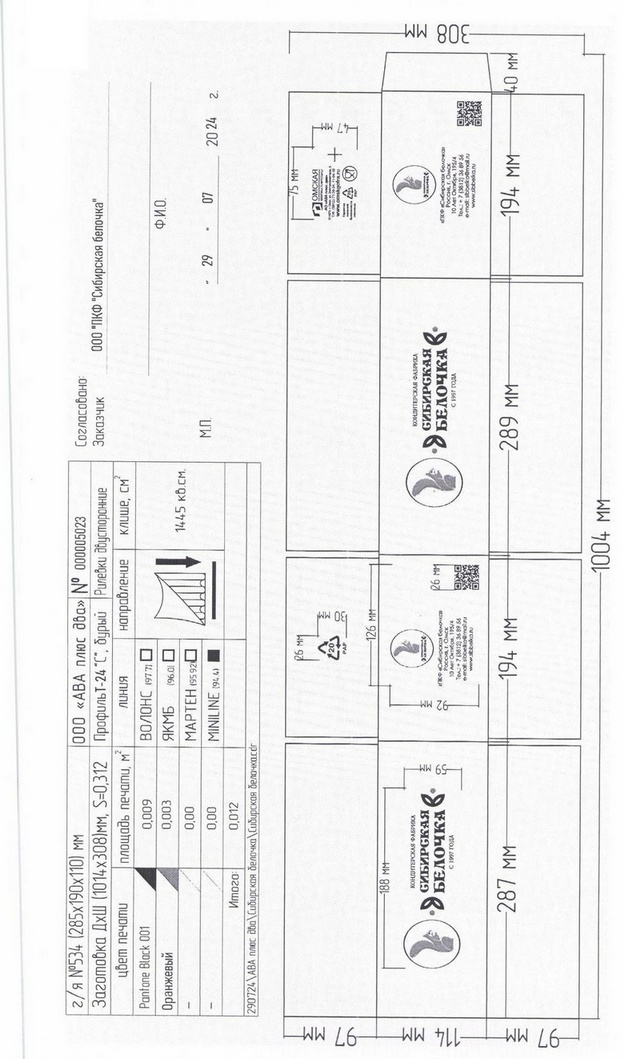
\includegraphics[height=0.94\textheight, width=0.94\textwidth, keepaspectratio]{Pics/d17.jpg}
\end{center}
  \caption{Форма макета ФПФ}
  \label{pic:d17}
\end{figure}


\begin{figure}
\begin{center}
  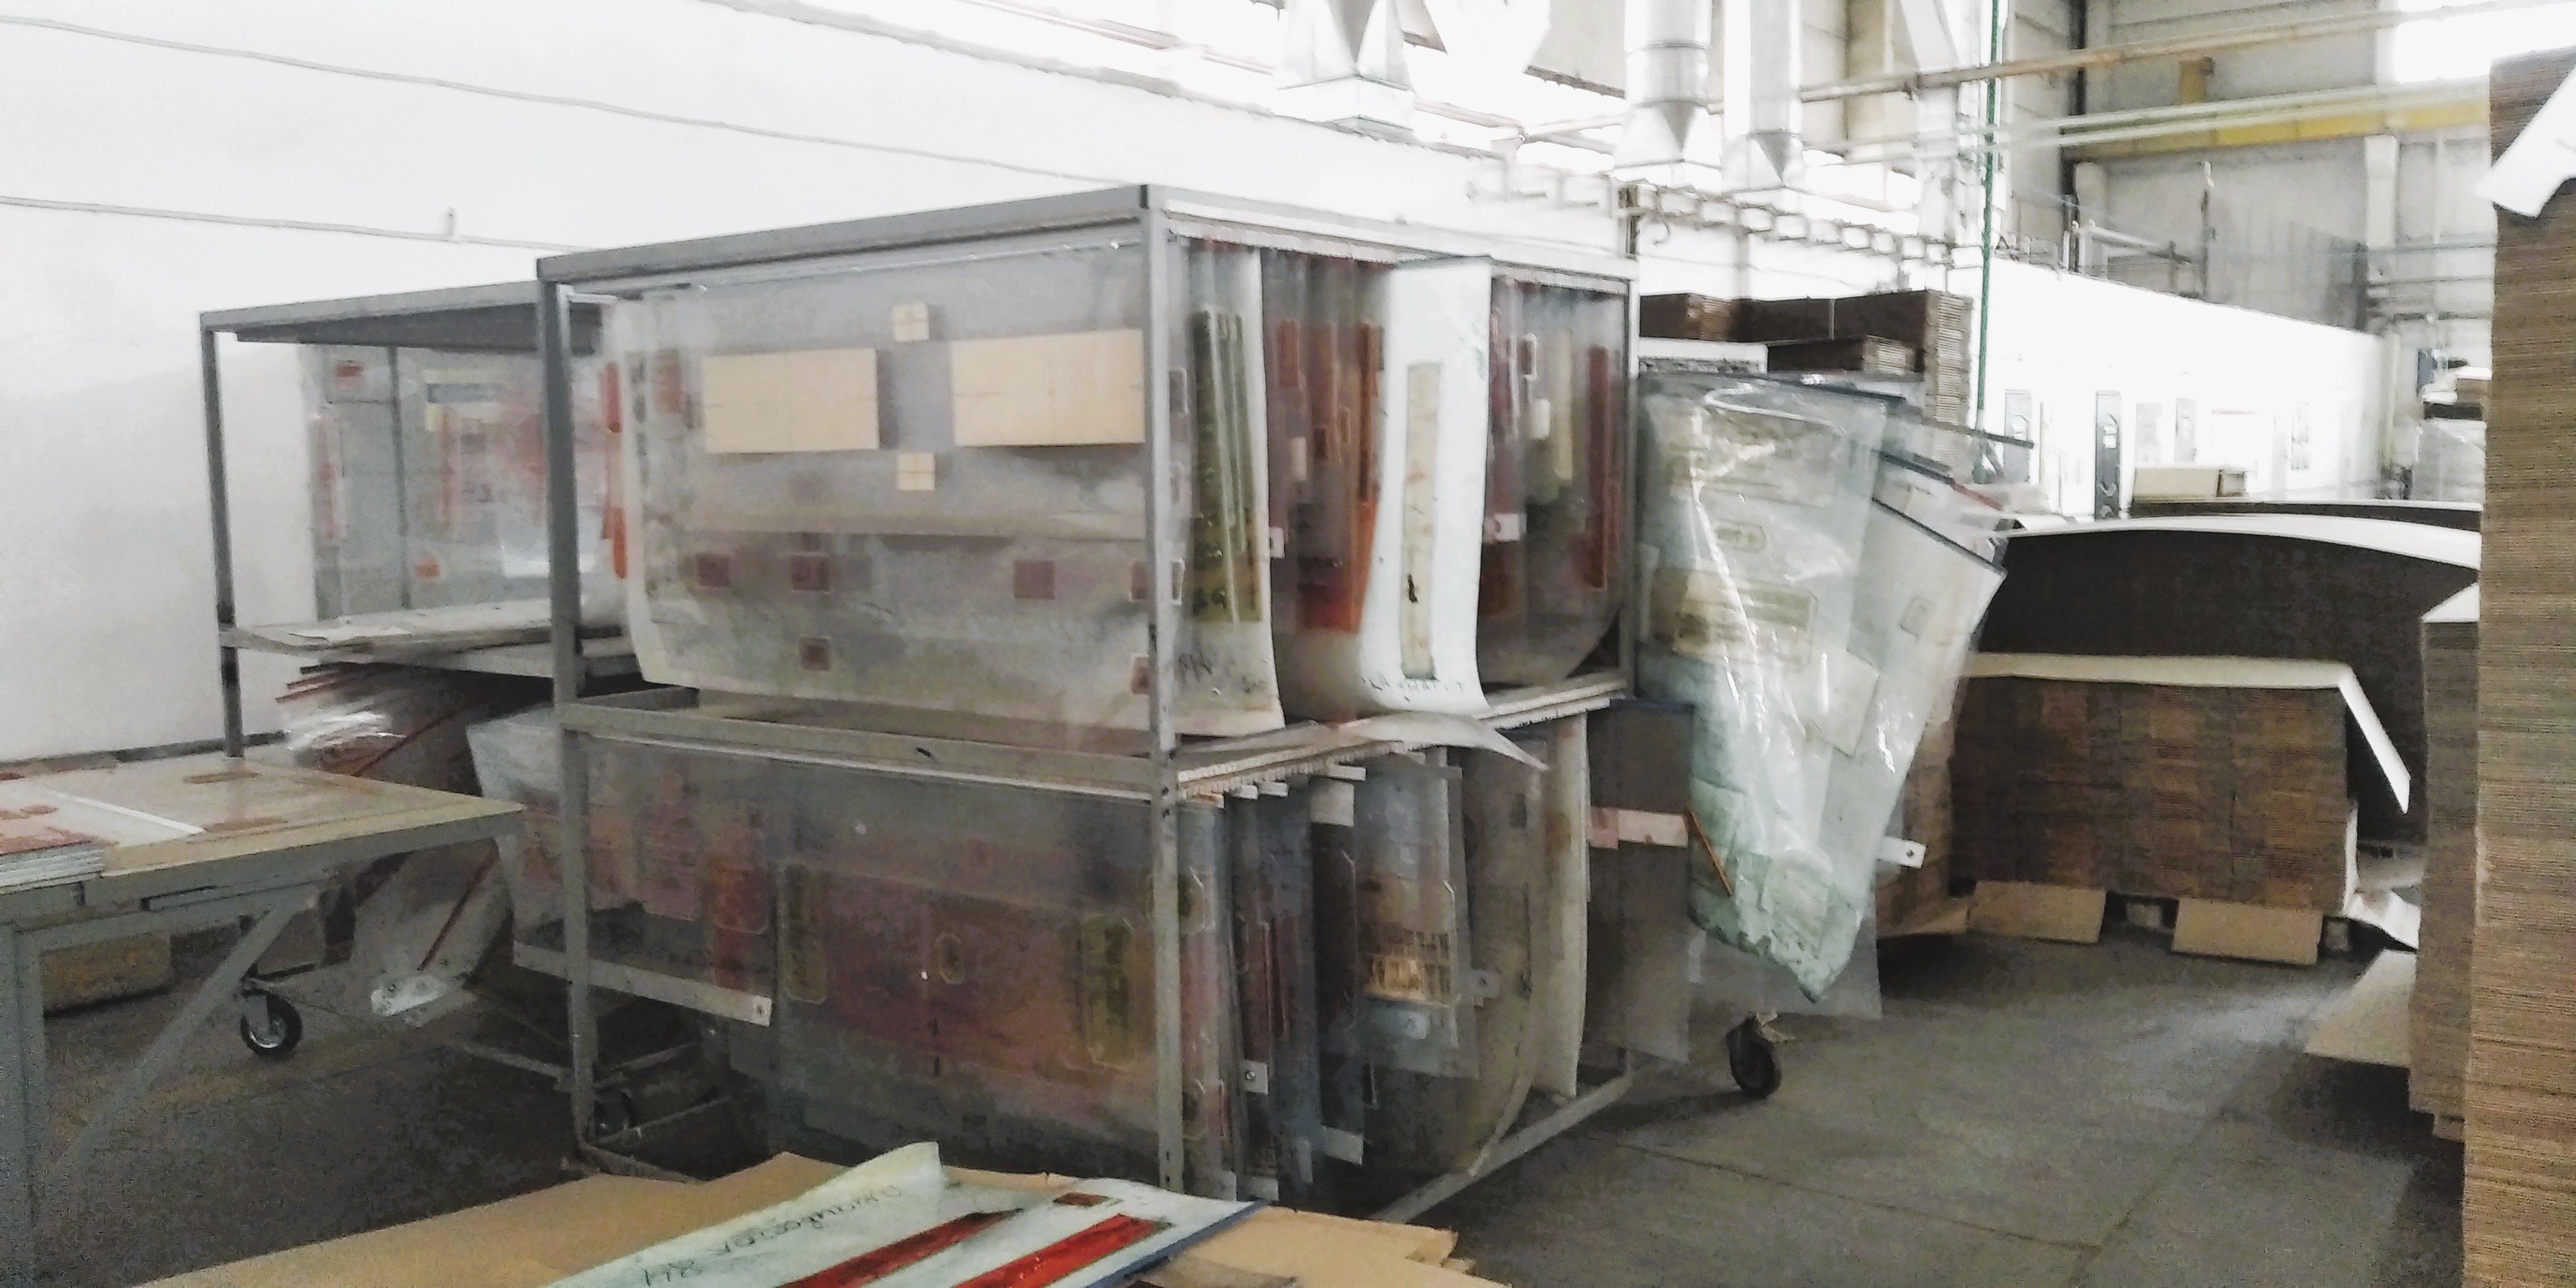
\includegraphics[height=0.94\textheight, width=0.94\textwidth, keepaspectratio]{Pics 1/6 хранение фпф.jpg }
\end{center}
  \caption{Место хранения ФПФ}
  \label{pic:1/6 хранение фпф}
\end{figure}

\begin{figure}
\begin{center}
  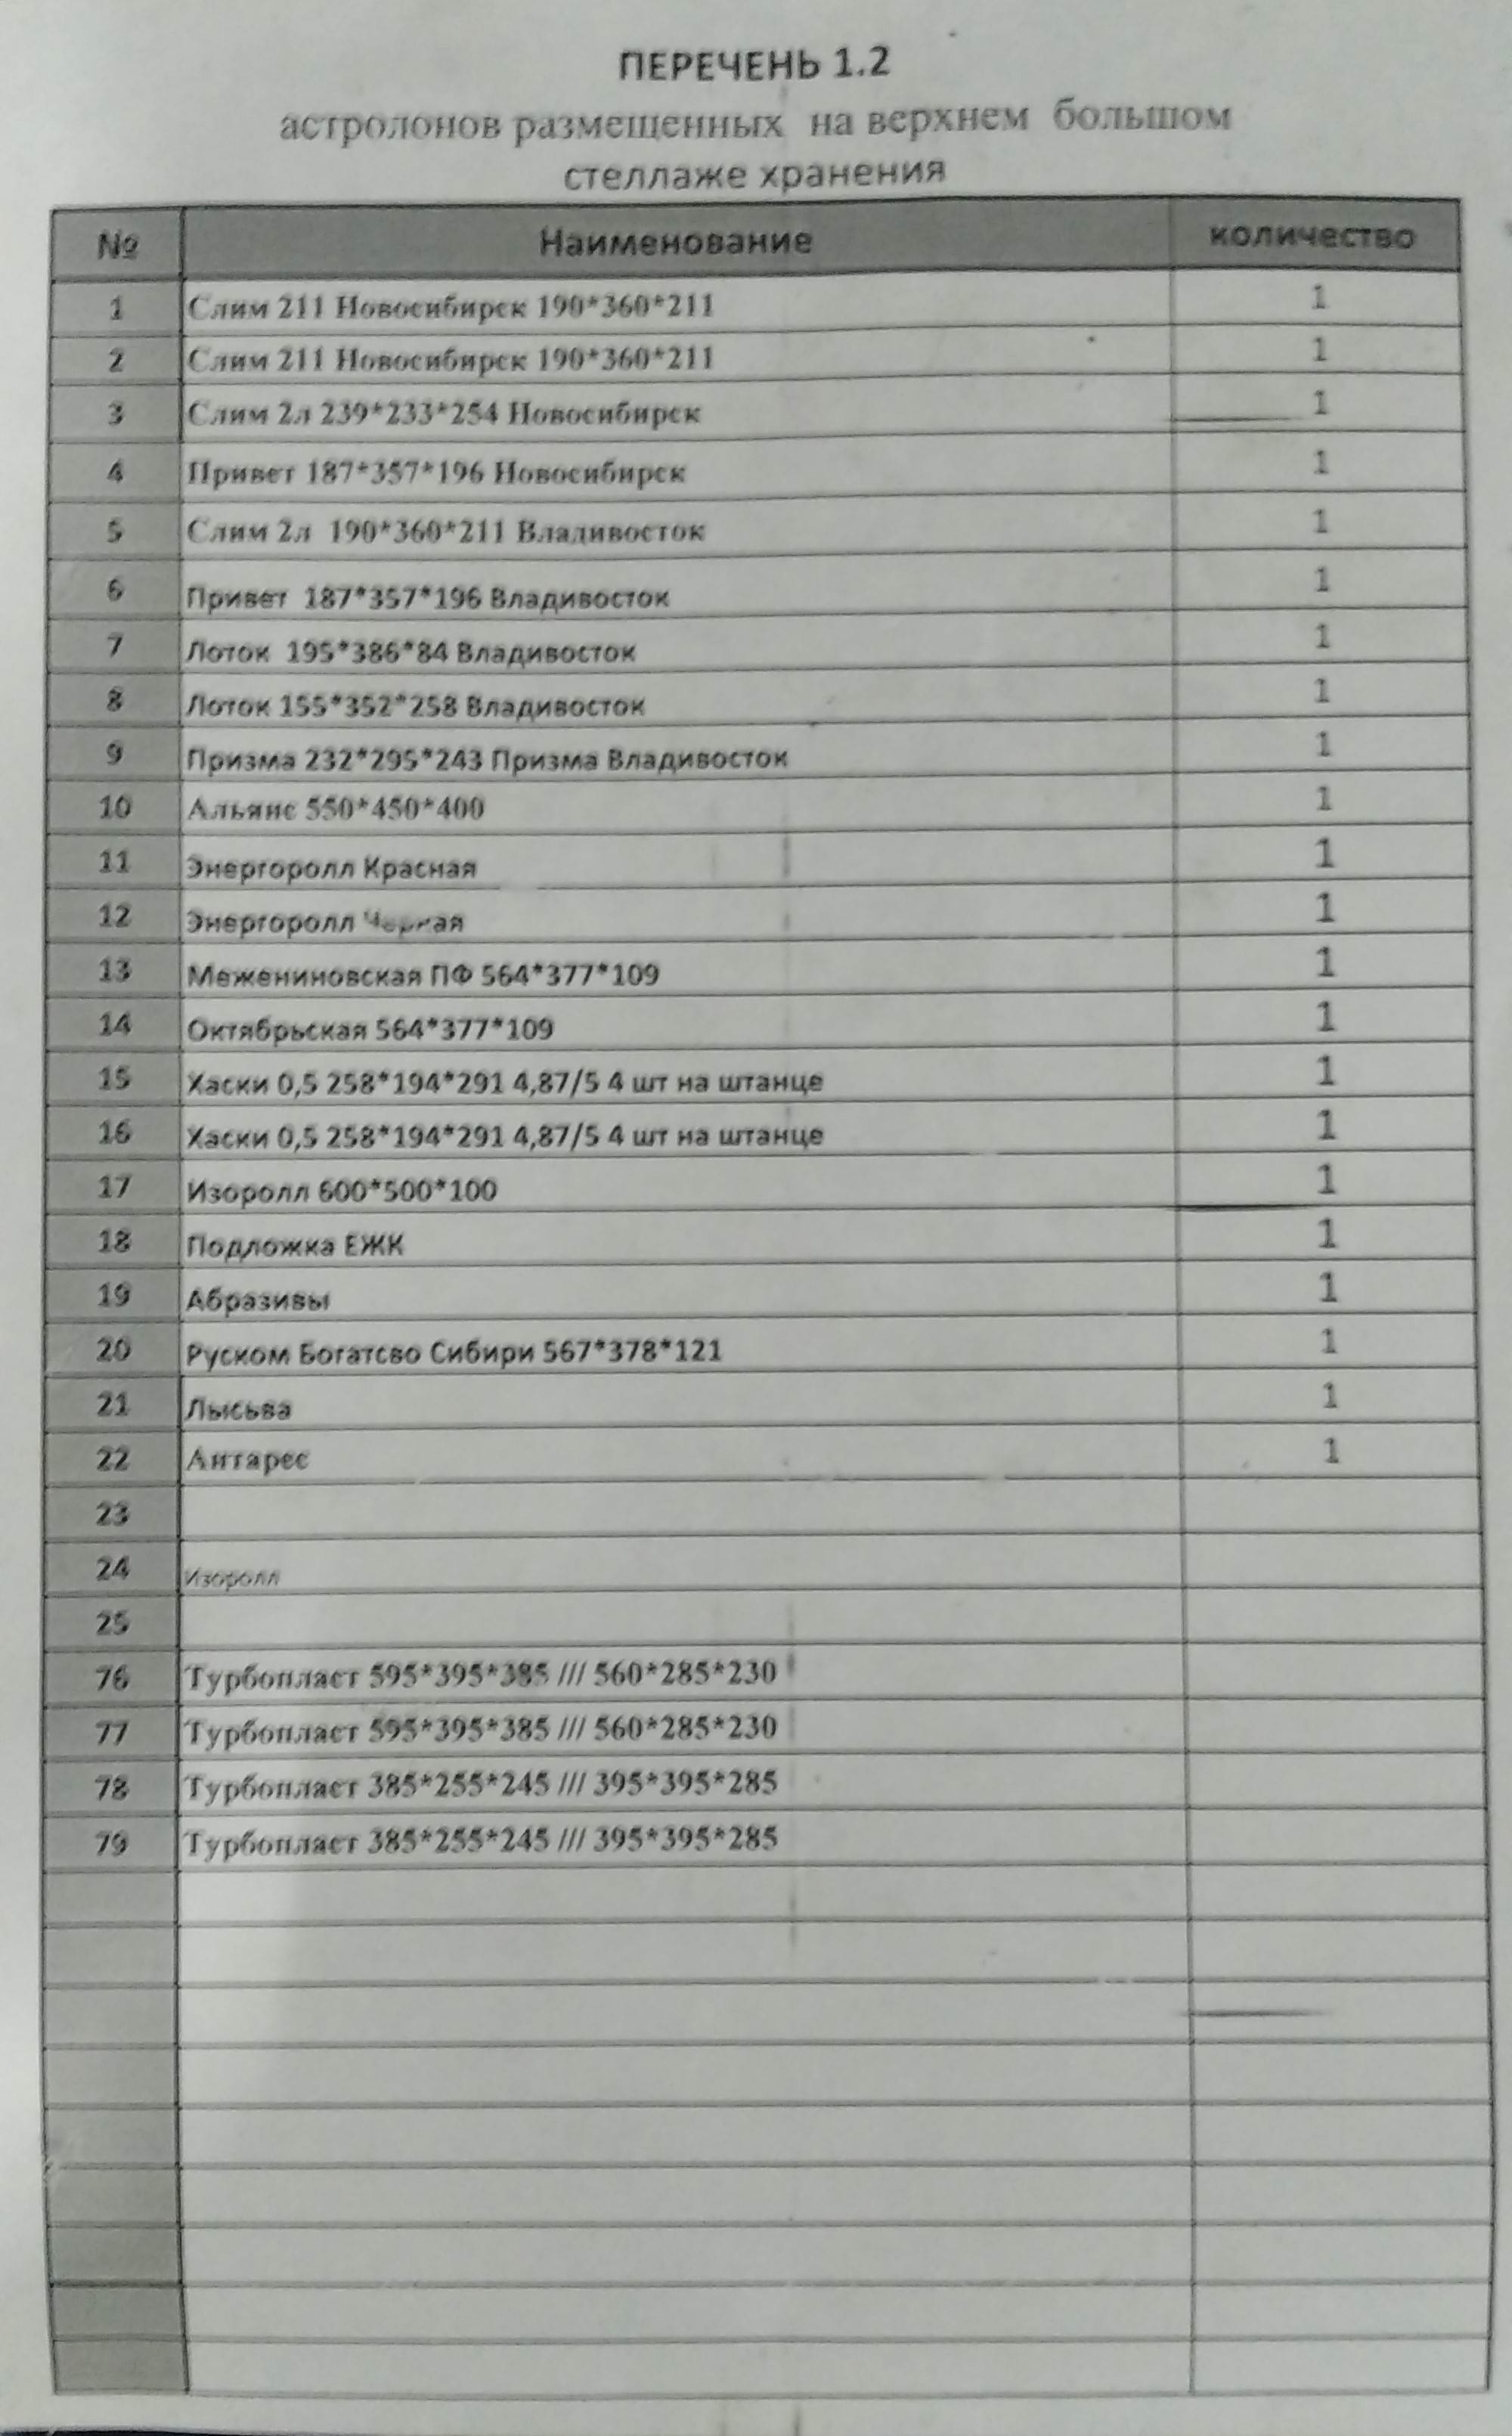
\includegraphics[height=0.94\textheight, width=0.94\textwidth, keepaspectratio]{Pics 1/6 перечень оснастки.jpg}
\end{center}
  \caption{Список печатных форм}
  \label{pic:1/6 перечень оснастки}
\end{figure}

\begin{figure}
\begin{center}
  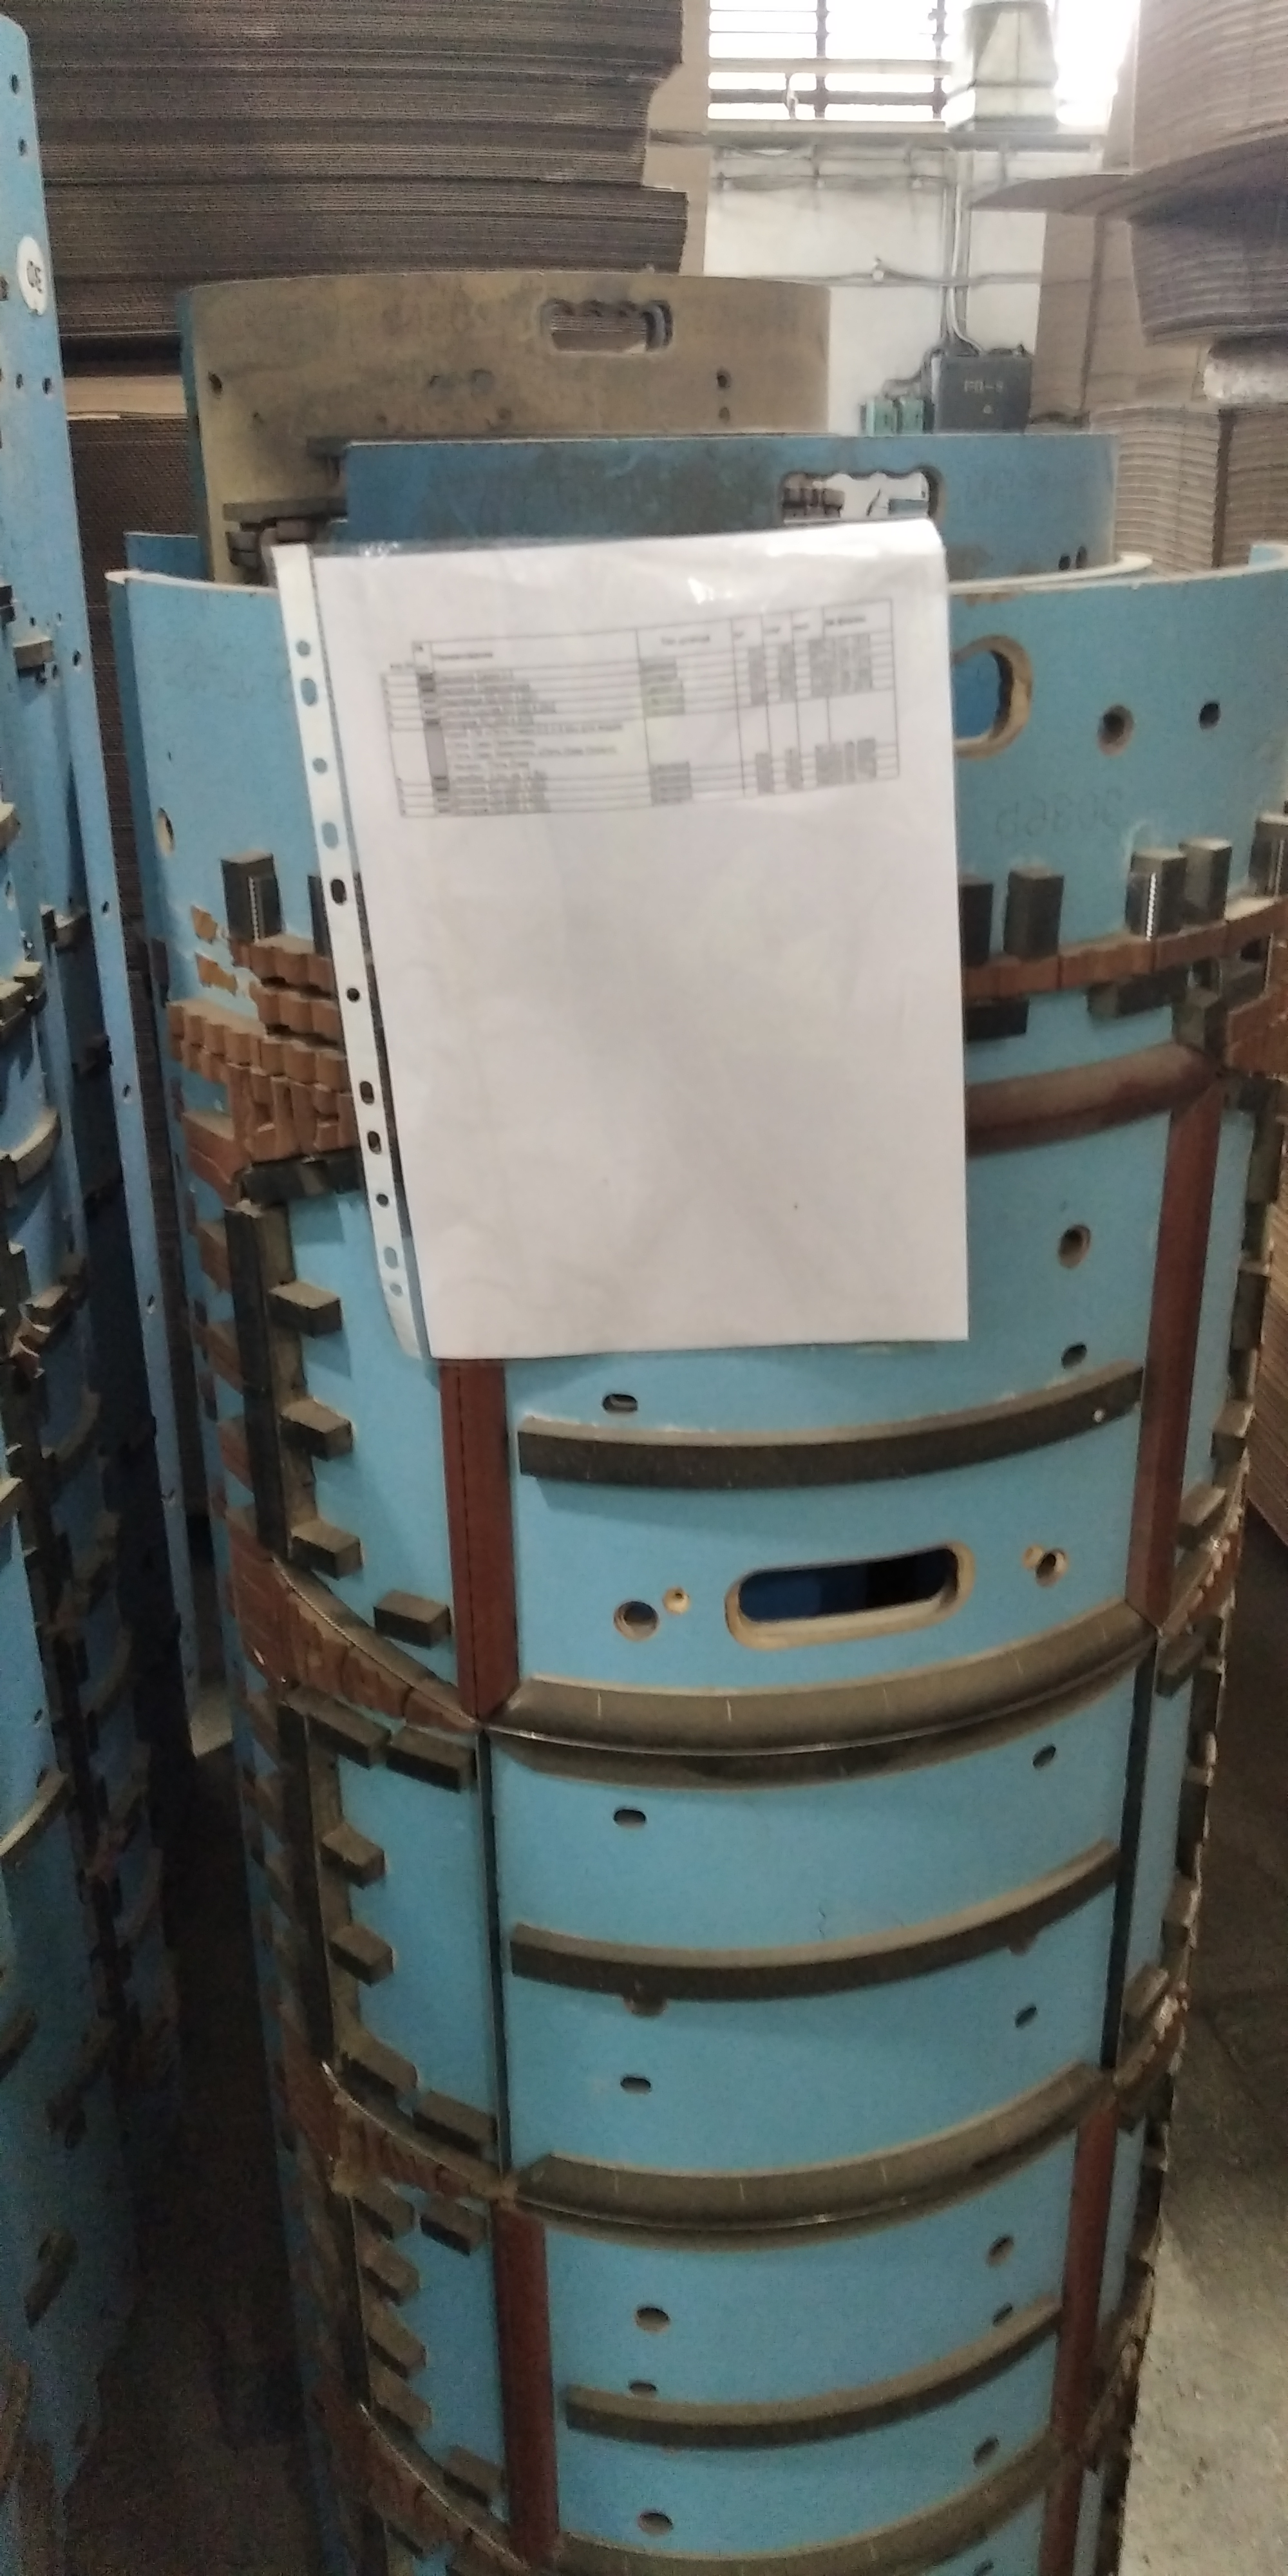
\includegraphics[height=0.94\textheight, width=0.94\textwidth, keepaspectratio]{Pics 1/6 хранение штанцев.jpg}
\end{center}
  \caption{Хранение штампов}
  \label{pic:1/6 хранение штанцев}
\end{figure}









 \begin{figure}
 \begin{center}
   
\includegraphics[height=0.94\textheight, width=0.94\textwidth, keepaspectratio]{Pics 1/1.8 приобретение оснастки_0001.jpg}
 \end{center}
   \caption{Служебная на приобретение оснастки}
   \label{pic:1.8 приобретение оснастки_0001}
 \end{figure}

% \begin{figure}
% \begin{center}
%   \includegraphics[height=0.94\textheight, width=0.94\textwidth, keepaspectratio]{Pics/a9.jpg}
% \end{center}
%   \caption{Отчет по поступлению краски}
%   \label{pic:a9}
% \end{figure}


%\begin{figure}
%\begin{center}
%  \includegraphics[height=0.94\textheight, width=0.94\textwidth, keepaspectratio]{Pics/f18.jpg}
%\end{center}
%  \caption{Хранение краски}
%  \label{pic:f18}
%\end{figure}

%\begin{figure}
%\begin{center}
%  \includegraphics[height=0.94\textheight, width=0.94\textwidth, keepaspectratio]{Pics/f19.jpg}
%\end{center}
%  \caption{Хранение краски}
%  \label{pic:f19}
%\end{figure}


% \begin{figure}
% \begin{center}
%   \includegraphics[height=0.94\textheight, width=0.94\textwidth, keepaspectratio]{Pics/pic_d41.jpg}
% \end{center}
%   \caption{Форма  оснастки монтажистам}
%   \label{pic:pic_d41}
% \end{figure}
% \clearpage
%
% 

\clearpage
\ifx \notincludehead\undefined
\normalsize
\end{document}
\fi
